\section{S2Store Ecosystem}
\label{sec:s2store_ecosystem}

The S2Store ecosystem like most ecosystems is expected to grow over time as the developers, their contributions and the number of users downloading them increase. The interaction becomes complex relationships, filling niches, competing and cooperating, similar to species in a biological ecosystem \cite{lim2012successful}. Ecosystem health is dependent upon community of developers that create innovative solutions that users want to use and the users providing relevant feedback back to the developers. The S2Store, central to the ecosystem allows anyone to build and publish their services. 

\begin{figure}[!htb]
  \centering
  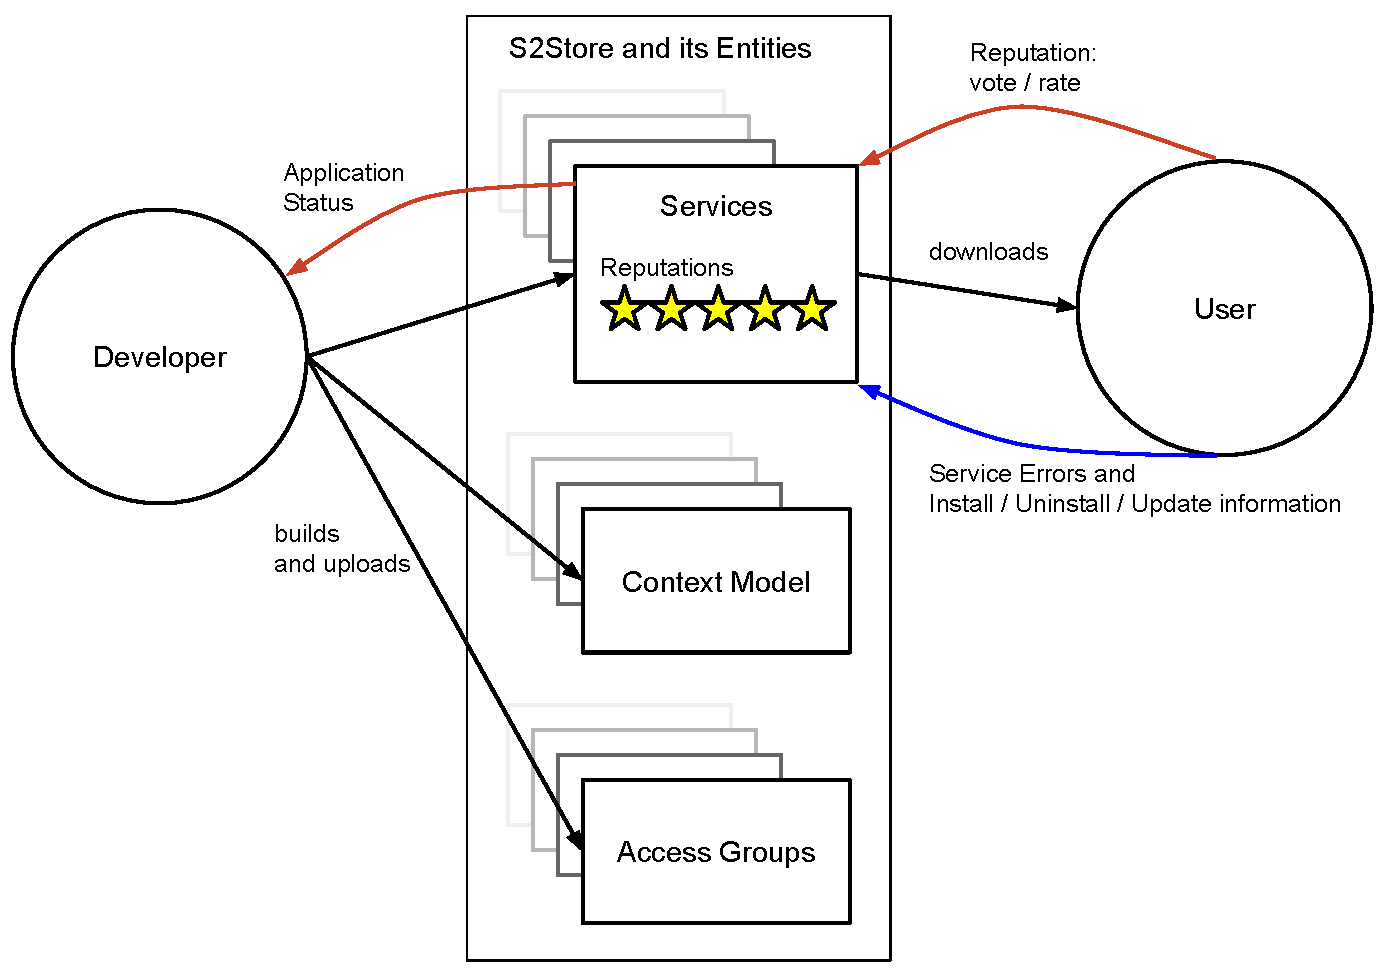
\includegraphics[width=15cm]{figures/ecosystem.pdf}
  \caption{Interaction between developers, entities and users in S2Store ecosystem.}
  \label{fig:ecosystem}
\end{figure}

\subsection*{S2Store Ecosystem Components}

S2Store ecosystem consists of developers, entities (context models, access groups and services) repositories and the users. Each component is described in detail below.

\subsection{Developers}

A developer is a registered user on the S2Store website who submits an application to the S2Store. Upon registration as a developer, she receies a \emph{developer-id} that is used to sign the application before submission. The developer-id is auto generated by the S2Store and unique per developer.

When creating a service for a smart space, a developer has to add the following entities:

\begin{itemize}
  \item Context-models that abstract the real world sensors or actuators or behaviors of desired smart space.
  \item Access-groups that group a set of resources and used to provide or revoke user permissions on these resources.
\end{itemize}

Context models and access groups are defined in Section \ref{subsubsec:context_model} and \ref{subsec:access_groups_and_convergence}. For both context models and access groups, a developer first searches if they exist already. When a suitable entity is found, a developer can reuse them in the service she develops. In case a suitable entity is not found, she can define new access groups and create new context models, submit to the S2Store and use them in her application.

The developer attaches a cryptographic signature to the application and submits it to S2Store. Once an application is marked as published, other users can download and install immediately.

A developer have access to multiple feedbacks collected by S2Store. She can see the statistics e.g. number of downloads, number of updates, removals, ratings by users. She can also see any comments and feedbacks submitted by users and respond back. S2Store can collect error logs submitted by applications and display them to developer so she can fix them.

A newer version of an application can be submitted to the S2Store. Users of old version are notified about the update.

\subsection{Context Model Repository}
\label{subsec:cmr}

Context Model Repository (CMR) deals with \emph{context models}. Context Models are briefly explained in the following section. We then explain their relationship with the CMR.

\subsubsection{Context Model}
\label{subsubsec:context_model}

A \emph{Context Model} is an abstraction of a context in a physical world into the virtual world. In VSL \si{\micro}-middleware, context models are expressed in XML.

\begin{lstlisting}[caption=A context model of a lamp., label=lst:lamp]
  <lamp>
    <isOn type="/derived/boolean">0</isOn>
    <dimLevel type="/basic/number" lowerBound="1" upperBound="5">3</dimLevel>
  </lamp>
\end{lstlisting}

The listing above is a context model of a real world lamp. It stores two attributes of a real world lamp: \texttt{isOn} and \texttt{dimLevel}. The default value for \texttt{isOn} is 0 - which relates to the lamp being turned off. The default value of \texttt{dimLevel} is 3 - which relates to the brightness level being in the middle of 1 and 5.

The VSL \si{\micro}-middleware reads these xml-templates of the context models and instantiates them with the default values. Services with either \emph{read} or \emph{write} permissions can perform respective activities on the context model instances. Permission and Security are explained in \ref{subsec:access_groups_and_convergence}.

\subsubsection{Context Model Hierarchy}

In VSL, context models form a hierarchical tree structure. The leaf nodes in the tree consist of three basic types provided by the system: number, string and list. The leaf nodes are \emph{inherited} to create complex sub-types. Advanced context models are created by \emph{composition} of simpler context models. In listing: \ref{lst:lamp}, a \texttt{lamp} definition is composed from another context models: \texttt{isOn} and \texttt{dimLevel}.

The following listing shows how a sub-type can be derived from the basic type.

\begin{lstlisting}[caption=Type inheritence: Sub type boolean is derived from /basic/number.]
  <boolean type="/basic/number" lowerBound="0" upperBound="1">
    0
  </boolean>
\end{lstlisting}

\subsubsection{Context Model Repository and Convergence}

The hierarchical tree structure of context models provides an additional benefit. Given a large number of developers involved in context modeling, we expect there would be a lot of duplicated effort. For e.g. multiple \emph{lamps} context models can exist from different developers or \emph{lamp1} could be of lesser quality than \emph{lamp2}.

The Context Model Repository is a central repository where developers can upload any context models they create. Each context model contains a globally unique identifier (guid). E.g. John can upload his context model at \texttt{/john/lamp1} and Jane can upload her context model at \texttt{/jane/lamp2}.

Other developers who want to program services for lamps can search for context model definitions of lamps. They see both John's and Jane's context models and decide on one of them.

With time, the number of context models increase in the CMR. Since context models link to each other, it forms a network that can be modeled with a directed graph. We can now calculate the importance of a context model in the global CMR space by analysing the number of forward associations and backward associations one context model has from its neighbours. The calculation of rankings of context models is explained in \ref{subsec:implicit_rating}.

Only developers interact directly with CMR, not the users. Developers can perform the following activities with the CMR:

\begin{description}
  \item[Validate:] A context model is dependent upon existing context models. CMR checks if the new context model definition is valid or not. It checks if the XML format is correct, whether the attributes passed to sub-nodes are correct, etc.
  \item[Upload:] A valid context model can be uploaded to the CMR. During upload, a developer requires the following information: \emph{xml, guid, tag set, description} where,

\begin{description}
  \item[xml] is the context model data.
  \item[guid] is the globally unique identifier. The scheme for the guid is similar to path structure for unix files and folders e.g. /username/device/abc/xyz/contextmodelname. First part of the guide is always namespaced with the username of the developer.
  \item[tag set] is a set of tags appropriate for the context model chosen by the developer.
  \item[description] describes the context model by writing what it is for, how it behaves and how others can use it. The description is used during full text search in the system. The rankings of the context models are dependent upon combination of internal and external reputation Section~\ref{sec:reputation_systems}.
\end{description}

\end{description}

% What are they, what do they do in DS2OS?
% How are they written. How do they interlink with others?
% How are access groups defined inside
% How services use these context models
% The relationship between context models and the CMR.
% How are they uploaded, deleted, downloaded and updated?

\subsection{Access Groups and Convergence}
\label{subsec:access_groups_and_convergence}

Any node in a context model metadata (xml) can be associated with certain access privilege by their authors. The privileges associated for read permission are \emph{readerIDs} and those associated for write permissions are \emph{writerIDs}.

\begin{lstlisting}[caption=Listing of lamp context model with \texttt{readerId} and \texttt{writerId} permissions.]
<lamp reader="lamp_readers" writer="lamp_writers">
  <isOn type="/derived/isOn" reader="*">
</lamp>
\end{lstlisting}

In the above listing, \texttt{lamp} context model defines two accessIds: \texttt{lamp\_readers} for read access and \texttt{lamp\_writers} for write access. Similarly the child node \texttt{isOn} has \texttt{*} as reader Id which signifies that it is publicly readable.

When building a service, a developer has to write the list of \emph{accessIds} her service is dependent upon. It is used by VSL to provide access control by comparing accessIds from the \emph{service certificates} with the Ids stored in the metadata of each context node.

Each context model developer is free to choose any accessId (readerId or writerId) for the nodes in the context model. Also, a developer can see the accessId associated with existing context models and reuse them.

Before submitting a context model to the S2Store, a developer should upload any new \emph{accessIds} with a human understandable description. Only then can she upload the context model. Otherwise the context model submission is considered invalid.

The convergence mechanism described earlier for context models also applies for the access groups. When significant amount of context models are uploaded in the CMR, comparably significant amount of accessIds are collected with their descriptions. This information is easily available to read online for other developers.

Multiple accessIds could account for the same security context. E.g. \texttt{lamp1} could offer \texttt{lamp\_reader1} and \texttt{lamp2} could offer \texttt{lamp\_reader2}. However, the more a specific context model is used, the more its access group becomes popular.

Popularity calculation is done through a reputation system discussed in Section~\ref{sec:reputation_systems}. Popularity affects the ranking where an access group appears during search.

\subsection{Service Store and Convergence}

Services in the DS2OS are analogous to apps in the Apple AppStore or Google PlayStore. They are written in Java and utilize a fixed application programming interface (API) provided by DS2OS to interact with the VSL. DS2OS provides mechanisms for managing services within a Smart Space through Service-to-Space (S2S) Section~\ref{sec:ds2os}. Services can perform various different activities and are classified accordingly into following classes \cite{pahl2014distributed}:

\begin{enumerate}
  \item \textbf{Adaptation Services} connect Smart Devices to the VSL.
  \item \textbf{Advanced Reasoning Services} infer new context from existing VSL context.
  \item \textbf{Emulator Services} emulate the behavior of a service, e.g. an adaptation service that interfaces a Smart Device.
  \item \textbf{Remote Access Services} provide access to functionality in a remote DS2OS site.
  \item \textbf{User interface Services} provide a User Interface (UI) for DS2OS services.
  \item \textbf{Primary context providers} extend the semantics that can be used to identify context nodes.
\end{enumerate}

The different service classes reflect the wide variety of applications. The potential use cases for a service are vast.

Before a service is uploaded in the S2Store, the corresponding context model and access groups should also be uploaded. Then the service package is created that consists of the following contents:

\begin{itemize}
  \item \textbf{The service executable} An executable java package file in Java ARchive (JAR) format.
  \item \textbf{A service manifest file} contains basic information about the service e.g. unique service name, developer id, version number, cryptographic hash of the service executable, etc.
  \item \textbf{The service certificate} also contains some duplicate information as in the service manifest file but also contains additional fields like access groups (readerIDs and writerIDs) that it needs permission to, ModelId of the context model that belongs to the service, cryptographic hash of the context model and cryptographic hash of the manifest file.
\end{itemize}

The service package can now be finally uploaded to the S2Store.

\subsection{Users}

A user is someone interested in using the DS2OS to create smart spaces. Users download, configure and run the DS2OS their computing environments. DS2OS being a distributed system can run in multiple computing nodes. DS2OS provides an interface to interact with the packages in the S2Store. Users can perform the following activities:

\begin{itemize}
  \item \textbf{Browse} S2Store for top services or most recent services.
  \item \textbf{Search} S2Store for services according to users' preference and their available smart devices.
  \item \textbf{Install or Uninstall} a service and be able to run it or remove it.
  \item \textbf{Rate} a service according to the perceived quality.
  \item \textbf{Comment} about the service to send a public feedback.
\end{itemize}

\subsubsection{Browse}

Users can browse previously uploaded services in the S2Store by visiting the website. There are two lists that users can browse to discover new services.

\begin{itemize}
  \item \textbf{List 1: Recent Services} sorts the services by the date when they were uploaded. The recent uploaded services are displayed at the top.
  \item \textbf{List 2: Popular Services} sorts the services by the reputation ranking of the services. How reputation of a service is calculated is discussed in Section~\ref{sec:reputation_systems}.
\end{itemize}

In both lists, users are able to filter by the tags associated with the services. For e.g. a user can filter the listing to show services related with only \emph{lighting}.

\subsubsection{Search}

S2Store contains a search interface for users to browse existing apps. The interface is similar to those provided by existing mobile AppStores. E.g. Figure~\ref{fig:search-interface-play-store}

\begin{figure}[!htb]
  \centering
  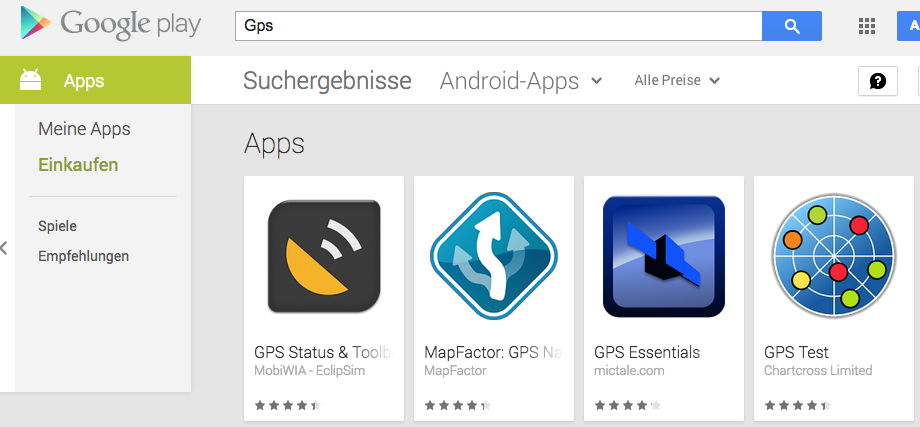
\includegraphics[width=14cm]{figures/search-interface-play-store.png}
  \caption{Search interface of Google's Play Store. (Source~https://play.google.com/store)}
  \label{fig:search-interface-play-store}
\end{figure}

% Search results are listed to the user according to a ranking algorithm discussed in \hl{TODO link to ranking algorithm discussion}

\subsubsection{Install or Uninstall}

DS2OS provides users with an interface to install a service into their local system. It will automatically download the software from the S2Store. Users can also keep track of available updates to existing services and uninstall them when necessary. Feedbacks are collected from these actions with the consent of the user. 

\subsubsection{Rate}

On the webpage of S2Store, users can rate any services they want. There exist different rating mechanisms discussed further in Section~\ref{sec:reputation_systems}. Ratings help to collect explicit feedback about a service from the users.

\subsubsection{Comment}

Comments are a common way to express user opinion on the internet. Comments serve multiple purposes in the S2Store. Users can comment to express satisfaction, dissatisfaction, request for new features in the service, report bugs, etc. Constructive comments help developers identify bugs and improve their services \cite{pagano2013user}.

\section*{Conclusion}

Reputation Systems in S2Store can bring convergence to hosted entities: services, context models and access groups. The Reputation Systems come in different varieties and one solution does not fit all. We analyzed and identified which models provides what kind of features and will look into how they suits S2Store.